\subsubsection{Adaptations to bit error rate training}
        
    In the previous progress report, the problem of training to minimize bit error rate (BER) instead of symbol error rate (SER) was tackled. The proposed approach was the addition of custom layers that converted from symbols to bits and vice versa. By training the neural network with and without these layers iteratively, The model was able to train to minimize BER. Even though this approach worked, it was quite bulky. A more elegant appraoch was implemented by defining a custom loss function:
    
    \begin{equation*}
        \mathcal{L} = SCE + \alpha \; BCE
    \end{equation*}
    
    where $SCE$ (Symbol Cross Entropy) is the categorical cross entropy computed on the softmax output representing the symbol predictions, $BCE$ (Bit Cross Entropy) is the elementwise binary cross entropy computed on sigmoid output representing the bit predictions and $\alpha$ is a weighting parameter to encourage training. Details of the loss function are given below:
    
    \begin{equation*}
        \begin{split}
            SCE &= \sum_{i}\sum_{j}-s_{ij}\log\hat{s}_{ij} \\
            BCE &= \sum_{i}\sum_{k}b_{ik}\log\hat{b}_{ik} + \left(1-b_{ik}\right)\log\left(1-\hat{b}_{ik}\right)
        \end{split}
    \end{equation*}
    
    where $i$ is the number of symbols being considered to compute the loss, $j$ is the number of elements in the softmax symbol prediction (i.e. the cardinality of the modulation scheme) and $k$ represents the number of bits per symbol. $s$ and $b$ are the true labels of the symbols and bits respectively while $\hat{s}$ and $\hat{b}$ are the symbol and bit predictions respectively. It should be noted that the symbol predictions are the output of a softmax layer and therefore do not directly predict the symbols but rather computes probabilities. \\
    \\
    Previously an attempt was made to train the model using just the $BCE$ metric which represents the bit error rate. However, this model did not converge to a solution well. This was overcome by using a weighted sum of the $SCE$ and $BCE$ metrics. 
    
\subsubsection{Spectrum analysis of encoded signal}
    
    \begin{figure}[H]
        \centering
        % 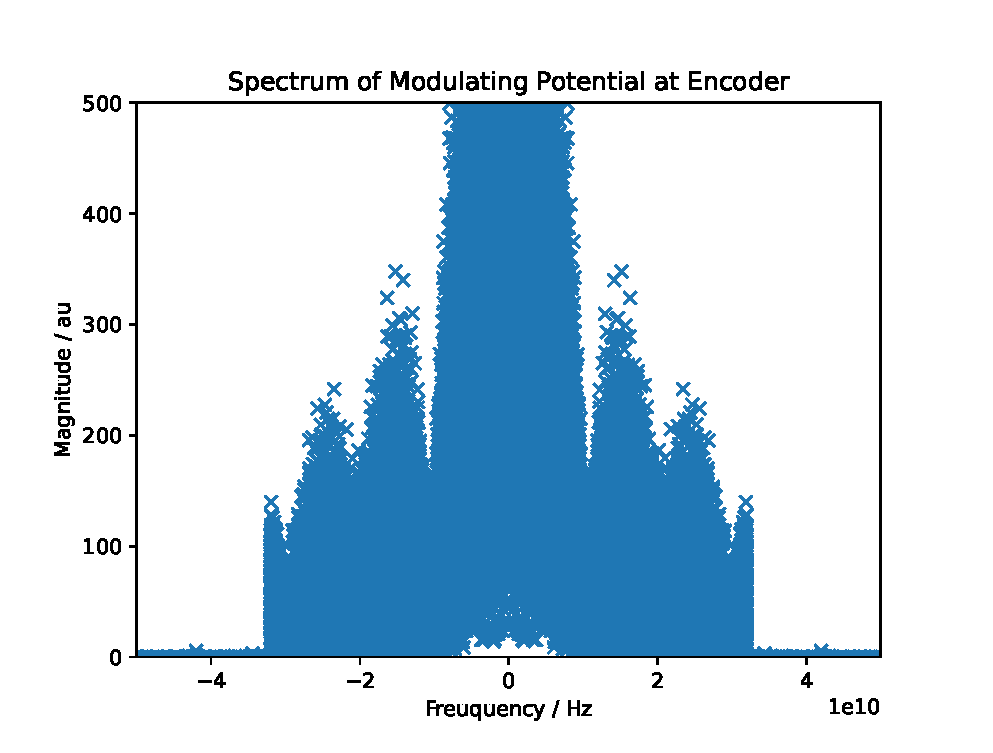
\includegraphics{nn_encoder_spectrum.eps} % Takes too long to load all data points on plot
        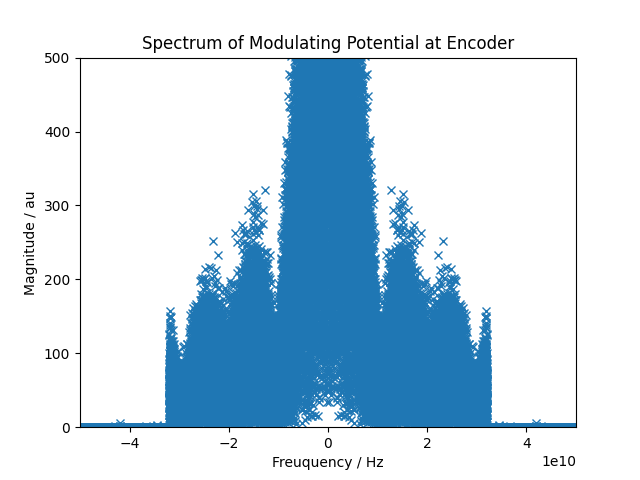
\includegraphics[width=0.8\linewidth]{nn_encoder_spectrum.png}
        \caption{Spectrum of the voltage potential modulating the laser light.}
        \label{fig:nn_encoder_spectrum}
    \end{figure}
    
    It was of interest to analyse the output signal of the encoder neural network. A table of learnt symbols was presented in a previous report but this report focuses on the frequency spectrum of the signal. Fig \autoref{fig:nn_encoder_spectrum} shows the frequency spectrum of the voltage potential used to modulate the laser light. Frequencies below above 32GHz are null due to the brickwall low pass filter. Besides the evident DC peak, further maxima and minima are also present. The minima occur at approximately 10 GHz, 20 GHz and 30GHz. We hypothesize that this blacklisting of frequencies learnt by the encoder neural network is to avoid frequencies at which the signal is null. Further analytical results are required to confirm this.
    
\subsubsection{Binary neural networks}
    
    As opposed to neural networks that use floating point values as weights and activations, a quantized binary neural network only has two states. A easy implementation of this is provided by the python library \textit{larq}. Many configurations were attempted but the model converged to a solution that had accuracies similar to random guesses. As the project is nearing it's end not too much time was spent on this and the approach was quickly abandoned. 